Como valores iniciales de las variables no observadas escogimos distintas opciones para asegurarnos de que no haya diferencia en los valores a los cuales convergen. Para los gráficos expuestos se utilizaron los siguientes parámetros para el algoritmo de muestreo.

\begin{lstlisting}[frame=single]
% Sampling
% MCMC Parameters
nchains = 2; % How Many Chains?
nburnin = 10e2; % How Many Burn-in Samples?
nsamples = 10e4;  %How Many Recorded Samples?
nthin = 1; % How Often is a Sample Recorded?
doparallel = 0; % Parallel Option

% Assign Matlab Variables to the Observed Nodes
datastruct = struct('k1',k1,'k2',k2,'k3',k3,'n',n);

% Initialize Unobserved Variables
for i=1:nchains
    S.theta1 = 0.5; % Intial Value
    S.theta2 = 0.8; % Intial Value
    S.theta3 = 0.5; % Intial Value
    S.alpha = randi([1 3]); % Intial Value
    init0(i) = S;
end

\end{lstlisting}

\subsection{Histogramas}

\begin{figure}[H]
\begin{minipage}{0.5\textwidth}
 \centering
	\includegraphics[width=1.2\textwidth]{imgs/alpha.pdf}
	\caption{\footnotesize Histograma de la variable $\alpha$.}
\end{minipage}
\begin{minipage}{0.5\textwidth}
 \centering
	\includegraphics[width=1.2\textwidth]{imgs/theta1.pdf}
	\caption{\footnotesize Histograma de la variable $\theta_1$. La linea azul es una aproximacion con una distribución normal.}
\end{minipage}
\end{figure}


\begin{figure}[H]
\begin{minipage}{0.5\textwidth}
 \centering
\includegraphics[width=0.9\textwidth]{imgs/theta3.pdf}
	\caption{\footnotesize Histograma de la variable $\theta_3$. La linea azul es una aproximacion (Poco precisa como se podrá observar)con una distribución normal.}
\end{minipage}
\begin{minipage}{0.5\textwidth}
 \centering
\includegraphics[width=0.9\textwidth]{imgs/theta2.pdf}
	\caption{\footnotesize Histograma de la variable $\theta_2$. La linea azul es una aproximacion con una distribución normal.}
\end{minipage}
\end{figure}

\subsection{Correlaciones}


\begin{figure}[H]
\begin{minipage}{0.5\textwidth}
 \centering
	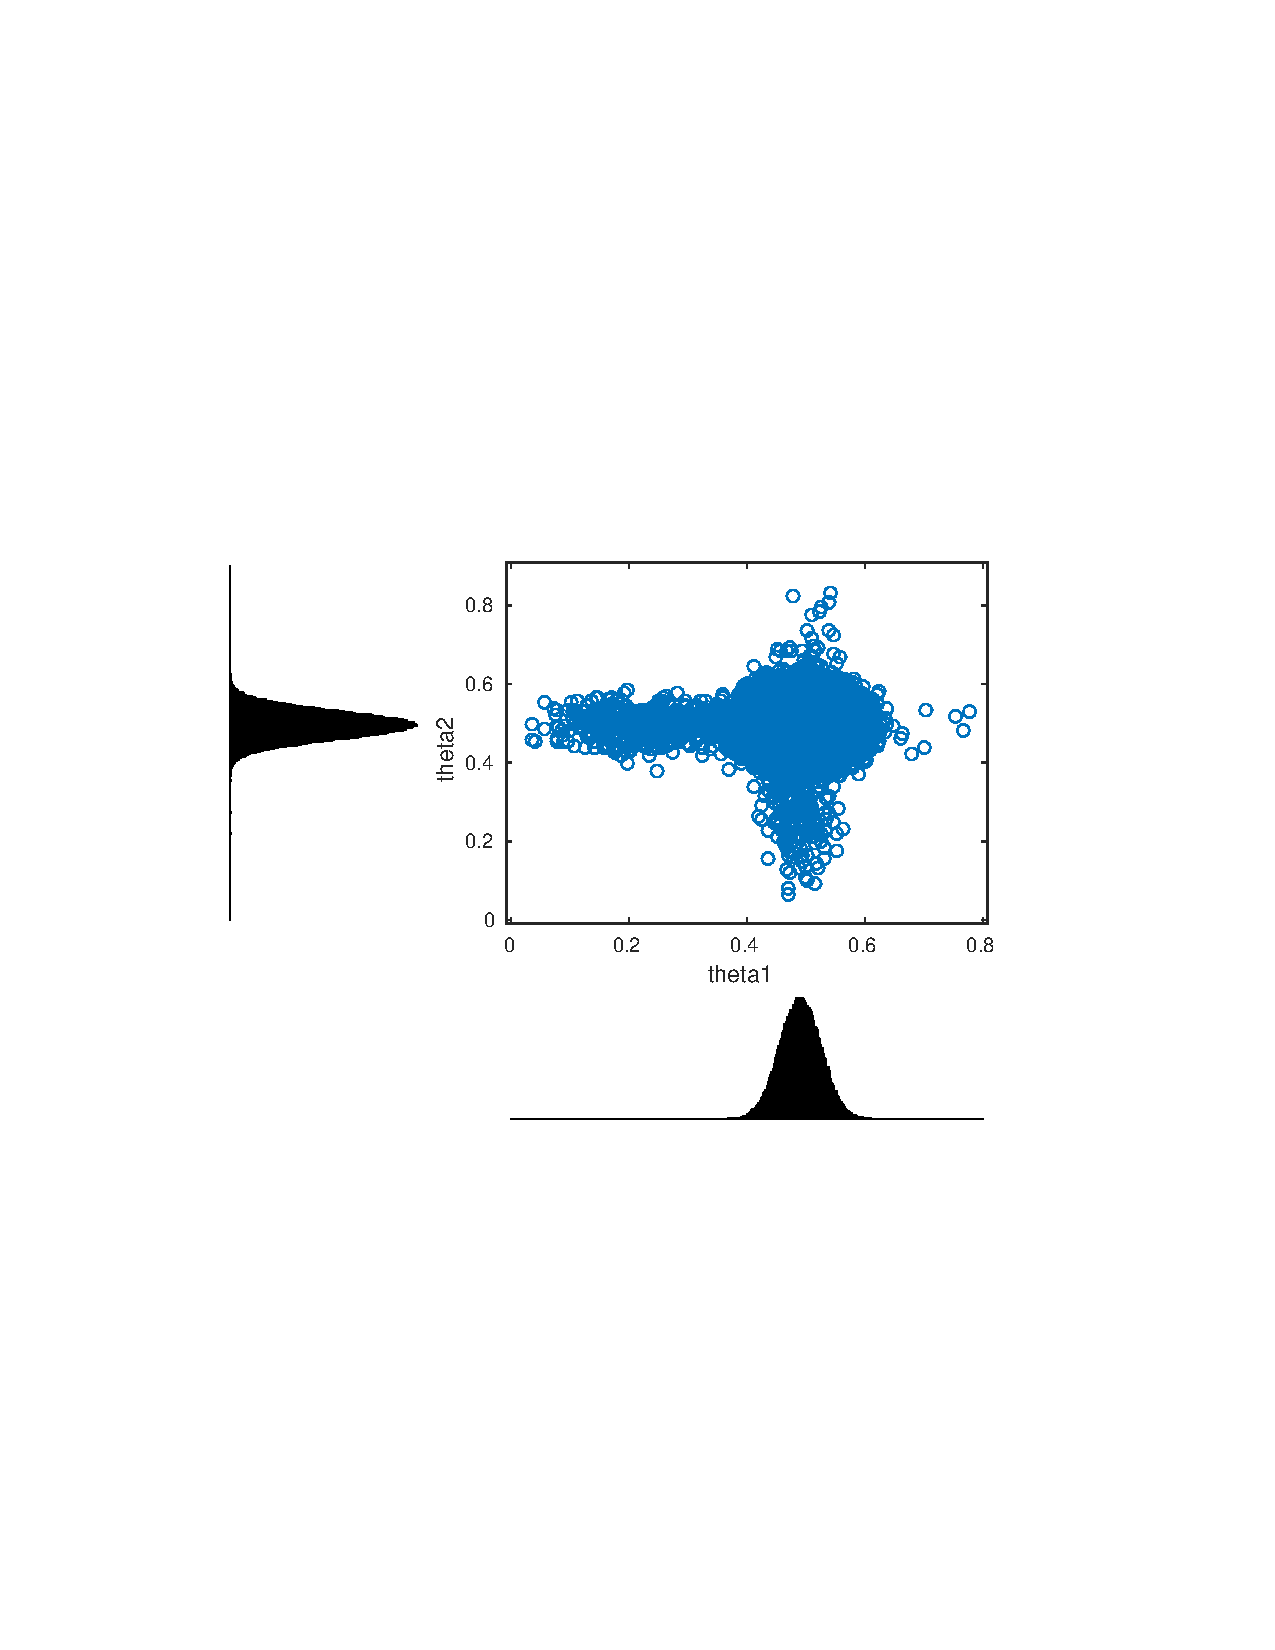
\includegraphics[width=0.9\textwidth]{imgs/theta1_2.png}
	\caption{\footnotesize Correlación entre $\theta_1$ y $\theta_2$.}
	\label{fig:problema2-promedio}
\end{minipage}
\begin{minipage}{0.5\textwidth}
 \centering
	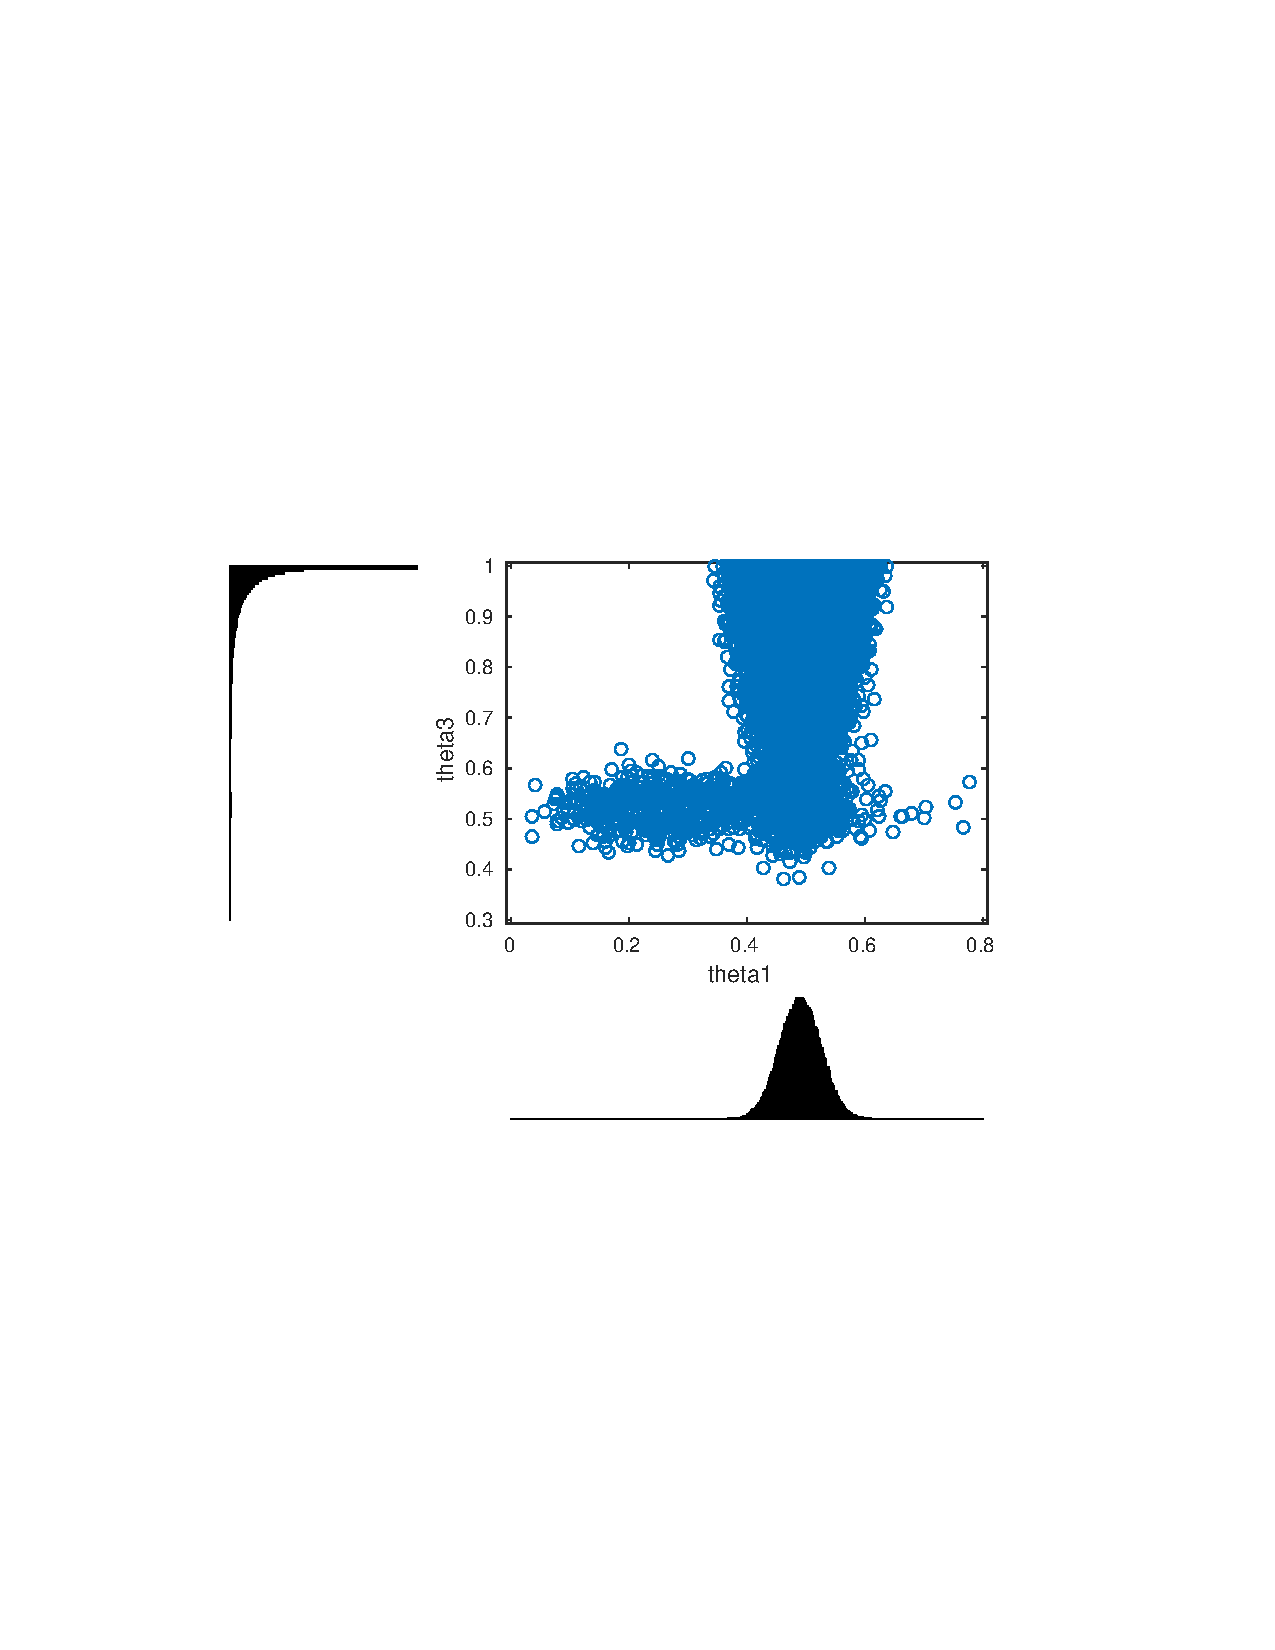
\includegraphics[width=0.9\textwidth]{imgs/theta1_3.png}
	\caption{\footnotesize Correlación entre $\theta_1$ y $\theta_2$.}
\end{minipage}
\end{figure}

\begin{figure}[H]
\centering
\begin{minipage}{0.5\textwidth}
	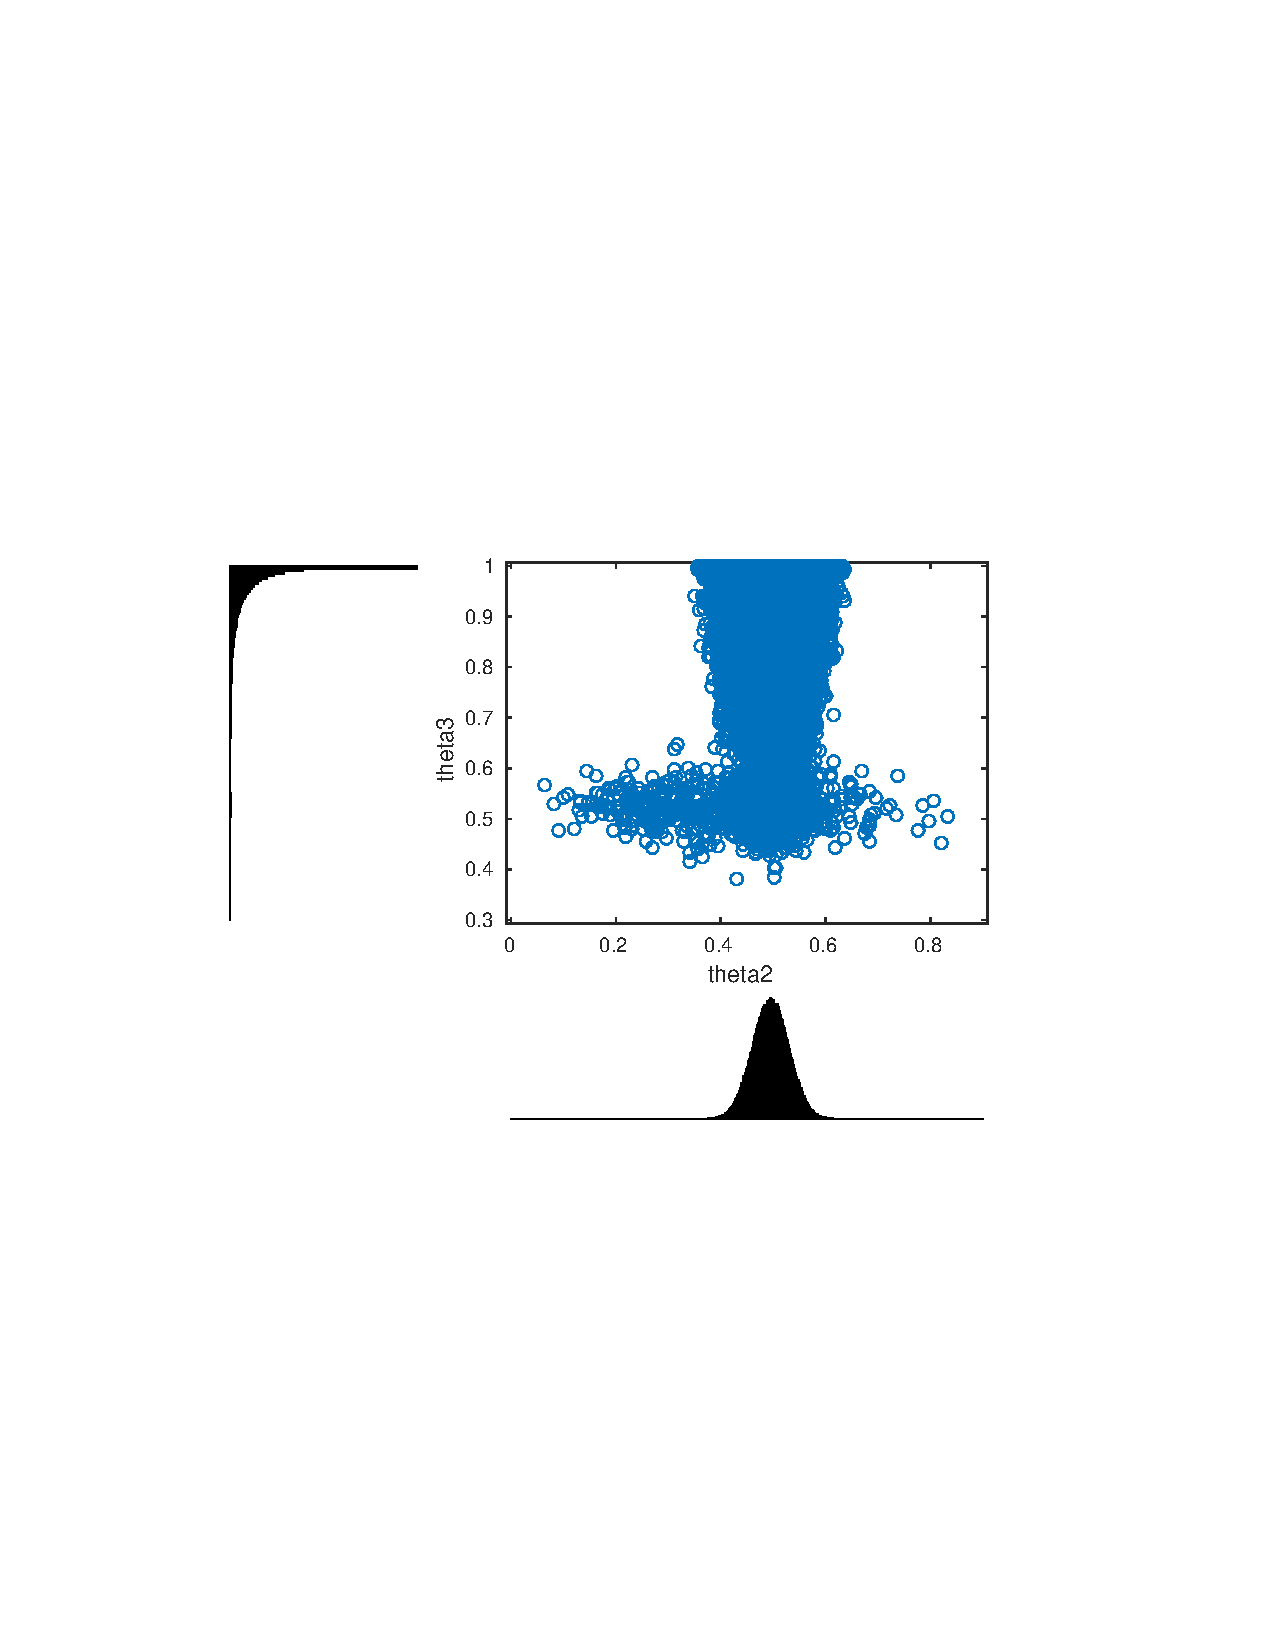
\includegraphics[width=0.9\textwidth]{imgs/theta2_3.png}
	\caption{\footnotesize Correlación entre $\theta_1$ y $\theta_2$.}
\end{minipage}	
\end{figure}


\subsection{Media y Desvío Standard}

media\_alpha = 2.9907

desvioStandard\_alpha = 0.1270

media\_t1 = 0.4899

desvioStandard\_t1 = 0.0368

media\_t2 = 0.4951

desvioStandard\_t2 = 0.0354

media\_t3 = 0.9523

desvioStandard\_t3 = 0.0680